\documentclass[11pt,letterpaper]{article}
% ---------------------------------------------------------------------------
% Preámbulo compartido (v2): tipografía, color, cuadros, figuras y cabeceras.
% Compilar con XeLaTeX. Todo lo que depende de papers.json llega por
% build/metadata.tex como macros semánticas (\papertitle, \paperauthors, ...).
% ---------------------------------------------------------------------------
\usepackage{fontspec}
% Serifa para el cuerpo: TeX Gyre Pagella (incluida en TeX Live completo).
\setmainfont{texgyrepagella}[Extension=.otf,UprightFont=*-regular,BoldFont=*-bold,
  ItalicFont=*-italic,BoldItalicFont=*-bolditalic,Scale=0.95]
% Sans para títulos, cuadros y figuras: TeX Gyre Heros.
\setsansfont{texgyreheros}[Extension=.otf,UprightFont=*-regular,BoldFont=*-bold,
  ItalicFont=*-italic,BoldItalicFont=*-bolditalic,Scale=MatchLowercase]
\setmonofont{Latin Modern Mono}[Scale=0.85]
\usepackage{polyglossia}
\setdefaultlanguage{spanish}
\setotherlanguage{english}
\usepackage[letterpaper,margin=27mm,headsep=7mm,footskip=11mm]{geometry}
\usepackage{microtype,graphicx,amsmath}
\usepackage{xcolor,placeins,etoolbox}
\usepackage{booktabs,tabularx,threeparttable,ragged2e}
\usepackage{enumitem}
\usepackage{titlesec}
\usepackage{caption}
\usepackage{fancyhdr}
\usepackage[hidelinks,unicode]{hyperref}
\usepackage{xurl}
\usepackage[autostyle]{csquotes}

% --- Paleta: un acento y un gris. Los cuadros permanecen en negro. -----------
\definecolor{tinta}{RGB}{23,59,54}    % acento (títulos, rótulos, trazos)
\definecolor{gris}{RGB}{107,107,102}  % cabeceras y notas discretas
\definecolor{humo}{RGB}{213,221,212}  % filetes muy suaves (solo figuras)

% --- Párrafo y página ----------------------------------------------------------
\linespread{1.04}
\setlength{\parskip}{0.3em}
\setlength{\parindent}{1.1em}
\setlength{\emergencystretch}{3em}
\tolerance=600 \hbadness=10000
\widowpenalty=10000 \clubpenalty=10000
\setlist{nosep}
\setcounter{secnumdepth}{3}

% --- Títulos de sección: sans, acento, numeración con punto (nivel 1) ---------
\titleformat{\section}{\sffamily\bfseries\large\color{tinta}}{\thesection.}{0.6em}{}
\titlespacing*{\section}{0pt}{1.6em}{0.6em}
\titleformat{\subsection}{\sffamily\bfseries\normalsize}{\thesubsection}{0.6em}{}
\titlespacing*{\subsection}{0pt}{1.1em}{0.35em}
\titleformat{\subsubsection}{\sffamily\itshape\normalsize}{\thesubsubsection}{0.6em}{}
\titleformat{\paragraph}[runin]{\itshape}{}{0pt}{}[.]

% --- Leyendas: rótulo en sans y acento, texto pequeño, alineado a la izquierda --
\captionsetup{font=small,labelfont={sf,bf,color=tinta},labelsep=period,
  justification=raggedright,singlelinecheck=false,skip=5pt}
\captionsetup[table]{position=above,skip=3pt}
\captionsetup[figure]{position=below}

% --- Cuadros: sans pequeña, sin líneas internas ni sombreado (guía del Boletín)
% Los flotantes reinician la fuente; el gancho correcto es \@floatboxreset.
\makeatletter
\g@addto@macro\@floatboxreset{\centering\ifdefstring{\@captype}{table}{\sffamily\small}{}}
\makeatother
\renewcommand{\arraystretch}{1.15}
\setlength{\tabcolsep}{5pt}
\setlength{\aboverulesep}{0.45ex}
\setlength{\belowrulesep}{0.65ex}
\newcolumntype{Y}{>{\RaggedRight\arraybackslash}X}  % texto, sin justificar
\newcolumntype{Z}{>{\RaggedLeft\arraybackslash}X}   % cifras alineadas a la derecha
\newcommand{\nd}{---}                               % dato no documentado
\newcommand{\aprox}{\ensuremath{\approx}}
\newcommand{\mayor}{\ensuremath{>}}
\newcommand{\menor}{\ensuremath{<}}
\newcommand{\cabecera}[1]{\textbf{#1}}              % cabecera de columna
\newcommand{\fila}[1]{\textbf{#1}}                  % rótulo de fila
% Notas al pie de cuadro: \begin{tablenotes}[flushleft]\footnotesize ... \end{tablenotes}
\appto\TPTnoteSettings{\footnotesize\color{gris}\RaggedRight}

% --- Cabecera y pie ------------------------------------------------------------
\pagestyle{fancy}\fancyhf{}
\renewcommand{\headrulewidth}{0pt}
\setlength{\headheight}{14pt}
\fancyhead[L]{\footnotesize\sffamily\color{gris}\papershorttitle}
\fancyhead[R]{\footnotesize\sffamily\color{gris}%
  \ifdefstring{\paperstatus}{draft}{Borrador \textperiodcentered{} fuentes: \sourcerevision}{}}
\fancyfoot[C]{\small\sffamily\thepage}
\fancypagestyle{plain}{\fancyhf{}\renewcommand{\headrulewidth}{0pt}%
  \fancyfoot[C]{\small\sffamily\thepage}%
  \fancyhead[R]{\footnotesize\sffamily\color{gris}%
    \ifdefstring{\paperstatus}{draft}{Borrador \textperiodcentered{} fuentes: \sourcerevision}{}}}

% --- Bloque de título (datos desde build/metadata.tex) -------------------------
\newcommand{\paperheading}{%
  \thispagestyle{plain}%
  \begin{center}
    {\sffamily\bfseries\Large\color{tinta}\papertitle\par}\vspace{0.55em}
    {\itshape\papertitleen\par}\vspace{1.2em}
    {\paperauthors\par}\vspace{0.45em}
    {\small\paperaffiliations\par}\vspace{0.25em}
    {\small\color{gris}Correspondencia: \papercontact\par}
  \end{center}
  \vspace{0.3em}{\color{tinta}\hrule height 0.5pt}\vspace{1.1em}}

% --- Resúmenes y palabras clave: medida algo más estrecha, rótulo en acento ---
\newenvironment{bloqueresumen}[1]{%
  \par\begingroup\small
  \setlength{\leftskip}{7mm}\setlength{\rightskip}{7mm}\setlength{\parindent}{0pt}
  \noindent{\sffamily\bfseries\color{tinta}#1.}\enspace\ignorespaces}{\par\endgroup}
\newcommand{\clave}[2]{\par\begingroup\small
  \setlength{\leftskip}{7mm}\setlength{\rightskip}{7mm}\setlength{\parindent}{0pt}
  \noindent{\sffamily\bfseries\color{tinta}#1:}\enspace #2\par\endgroup\medskip}

% --- Compatibilidad con el verificador: el banner ya no se invoca en el cuerpo --
\newcommand{\draftnotice}{}
\newcommand{\editorialtodo}[1]{\textbf{[Revisión editorial: #1]}}

\input{build/metadata}
\begin{document}
\paperheading
\begin{bloqueresumen}{Resumen}El acceso abierto a recursos científicos requiere organización para sostener la participación. Este ensayo compara CoAfina, el editatón Salud para todos con la OMS y Cornell, y experiencias venezolanas con ATLAS Open Data. Una síntesis documental distingue inscripción, actividad, productos y continuidad. Recuperamos resultados públicos de tres ediciones de CoAfina, definiciones y metas publicadas del editatón, y cocientes descriptivos con sus límites. Los editatones registran cocientes de actividad del 42,2\,\% y 26,5\,\%; los umbrales de otros formatos difieren e impiden comparar eficacia educativa. La documentación identifica ayudas asociadas a entregas, un canal comunitario que persistió y un paso de participante a proponente de retos. Una matriz relaciona estos mecanismos con preservación, reconocimiento y seguimiento. Proponemos reutilizar definiciones operativas, vincular cada producto a sus materiales y asignar responsabilidades posteriores. El marco ofrece decisiones adaptables a instituciones venezolanas sin confundir alcance, aprendizaje y continuidad.
\end{bloqueresumen}
\clave{Palabras clave}{ciencia abierta; comunidades científicas; hackatones; educación; América Latina.}
\begin{english}
\begin{bloqueresumen}{Abstract}Open access to scientific resources requires support and organization to become sustained participation. This essay compares CoAfina, the Health for All editathon involving WHO and Cornell, and Venezuelan training experiences using ATLAS Open Data. A documentary synthesis distinguishes products, recognition mechanisms, and pathways for continued engagement. Results include an edition-level CoAfina inventory and a matrix connecting the three formats to preservation, review, and follow-up. The analysis identifies complementary supports: connections between teams and challenges, editorial histories, and academic recognition. We propose organizing each activity around a verifiable contribution, a reusable deliverable, and an assigned follow-up responsibility. The framework offers decisions that Venezuelan institutions can adapt and a basis for collecting comparable evidence on participation and reuse.
\end{bloqueresumen}
\clave{Keywords}{open science; scientific communities; hackathons; education; Latin America.}
\end{english}
\section{Introducción}
Abrir un recurso científico permite acceder a él; construir una comunidad exige organizar su uso, revisión y continuidad. Esta diferencia importa para instituciones venezolanas que buscan conectar formación, participación pública e investigación con recursos limitados. La Recomendación de la UNESCO sobre Ciencia Abierta sitúa la participación y la cooperación junto al acceso al conocimiento \cite{unesco}. El concepto de comunidad de práctica permite analizar el aprendizaje como participación sostenida en actividades compartidas \cite{wenger}.

Este ensayo sostiene que una actividad abierta se convierte en infraestructura comunitaria cuando deja tres elementos vinculados: una contribución identificable, un mecanismo de reconocimiento y una vía de continuación. La convocatoria y el número de asistentes describen el alcance de un encuentro, pero su continuidad se juega en las responsabilidades y recursos que quedan después. La revisión de Schulten y Chounta muestra que los estudios sobre aprendizaje en hackatones recurren con frecuencia a percepciones y carecen de procedimientos suficientemente estandarizados de evaluación \cite{hacklearning}. Por ello proponemos examinar productos y mecanismos concretos antes de atribuir efectos educativos.

Comparamos tres formatos: CoAfina, la edición colaborativa de conocimiento sanitario y la formación con datos abiertos de física. La contribución del ensayo es una matriz de decisiones que distingue lo que cada formato conserva, cómo reconoce el trabajo y qué necesita para prolongarlo. CoAfina es uno de los casos de una trayectoria más amplia de ciencia abierta en América Latina.

El mapeo de Costa, García-Holgado y Alvarez organiza marcos metodológicos, estructuras de organización y métricas de hackatones estudiantiles, y señala límites en su seguimiento longitudinal \cite{hackmapping}. Estas dimensiones fundamentan la separación entre organización, productos y continuidad en nuestra matriz.

\section{Enfoque y materiales}
\subsection{Selección y tratamiento de los casos}
Se realizó una lectura dirigida de documentación pública y de materiales proporcionados por los autores. La selección es intencional: incluye experiencias en las que las prácticas abiertas conectan conocimientos especializados con participación distribuida. Las unidades de análisis son la actividad y sus mecanismos organizativos, no los individuos. Se consideran tres formatos: un hackatón de datos, un editatón bilingüe y trayectorias educativas con datos de física.

El informe de CoAfina 2023 describe una actividad virtual con estudiantes universitarios y tareas de análisis \cite{coafina}. El artículo de Salud para todos aporta un registro publicado de edición colaborativa \cite{salud}. El relato de ATLAS sobre educación en Venezuela documenta el uso de datos abiertos en tesis y acompañamiento académico \cite{atlas}. Estos documentos no constituyen una muestra representativa de América Latina. Su lectura conjunta sirve para identificar mecanismos y formular preguntas que deberán contrastarse en otros contextos.

Para cada caso se distinguen: propósito, forma de participación, producto, apoyo especializado, condiciones de reutilización y evidencia de continuidad. Los números se conservan con su unidad original. Inscripción, edición, equipo y tesis no son categorías intercambiables. No se suman cohortes sin identificar participantes repetidos, ni se interpretan visitas a una página como aprendizaje. El registro de evidencia adjunto identifica la procedencia de cada afirmación y los puntos que requieren revisión de los autores.

\subsection{Alcance de la comparación}
La comparación es analítica, no una clasificación de eficacia. Un hackatón puede priorizar exploración, mientras una tesis exige un compromiso temporal y una evaluación diferentes. La pregunta relevante no es qué formato produce más participantes, sino qué combinación de tareas, apoyo y recursos hace posible una contribución verificable. La cercanía de los autores a las experiencias aporta conocimiento operativo, pero también introduce selección y posibles sesgos favorables; por ello se explicitan los límites de las fuentes.

El presente texto no incorpora entrevistas nuevas, encuestas individuales ni seguimiento longitudinal. Sus propuestas de evaluación son prospectivas. Los resultados publicados de otros trabajos se citan como antecedentes; en particular, el estudio de Salud para todos conserva su identidad y autoría propias. La contribución nueva de esta síntesis es la articulación entre formatos y el diseño de un marco común de documentación y continuidad.

\section{Resultados de la síntesis documental}
\subsection{CoAfina: alcance, productos y continuidad}
El informe de CoAfina 2023 registra 78 estudiantes, 16 equipos, 30 universidades y ocho países en una actividad virtual del 20 al 22 de octubre \cite{coafina}. La alianza organizadora incluyó LA-CoNGA physics, Creative Commons Venezuela, RedCLARA y CEDIA. El cuadro~\ref{tab:ediciones} separa ese recuento de las categorías necesarias para una comparación longitudinal. La convocatoria de 2024 identifica la tercera edición para el 19--21 de julio y comunica cerca de 150 estudiantes en ediciones anteriores; ese agregado no permite reconstruir inscripciones y finalización por año \cite{coafina2024}. La convocatoria archivada en el índice público para 2025 identifica una nueva edición, pero la página principal cambia con cada convocatoria \cite{coafina2025}.

\begin{table}[tbp]
\begin{threeparttable}
\caption{CoAfina por edición. Se conservan las unidades y los cortes temporales de cada fuente; una raya indica que no hay recuento documentado.}\label{tab:ediciones}
\input{build/ediciones-body}
\begin{tablenotes}[flushleft]
\item[a] Universidades de origen en el registro, no en la actividad final.
\item[b] 183 inscritos según la diapositiva de apertura de los organizadores (S1); corte de apertura, no actividad final ni registro individual depurado.
\item Actividad en 2022: aproximadamente la mitad de los inscritos; en 2023 y 2024, participantes reportados. En 2025 los siete retos corresponden a la apertura. Fuentes: \cite{coafina2022,coafina2023pre,coafina,uis2023,coafina2024,coafina2025,coafina2025apertura}.
\end{tablenotes}
\end{threeparttable}
\end{table}


La noticia de LA-CoNGA sobre 2023 enlaza demostraciones de soluciones y documenta el retorno de un participante de la edición anterior como proponente de un reto \cite{coafinacontinuidad}. Este es un ejemplo concreto de cambio de función dentro de la red. Las demostraciones conservan una explicación del producto; para verificar su ejecución futura se necesita además código, datos, dependencias y permisos. El hallazgo organizativo es que visibilidad del resultado y preservación ejecutable son tareas distintas, aunque ambas puedan formar parte de una misma entrega.

\subsection{Edición colaborativa con la OMS y Cornell}
El editatón de noviembre de 2021 conectó a OMS, Cornell, Wikimedia y Creative Commons. Su publicación de 2026 registra 45 inscritos de 12 países, 19 editores activos y 22 artículos nuevos; Creative Commons Venezuela aportó identidad visual y sitio bilingüe \cite{salud}. El artículo informa del reconocimiento concedido al equipo en 2022 por el Director General de la OMS en el desafío OMS LEAD 2021. La distinción reconoce la iniciativa; sus productos se identifican mediante ediciones.

Para el seguimiento, ALAN indica 2022; el boletín de Cornell anuncia ``Editathon V2: Health for All'' para el 13--16 de febrero de 2023 \cite{cornell}. Se mantienen separados ambos registros y se emplean únicamente las métricas de 2021 en la comparación.

Wikipedia aporta historial público y revisión posterior como parte de su plataforma. La literatura sobre su uso en salud destaca la importancia de participación experta y calidad de las fuentes \cite{wikihealth}. Para el diseño de un editatón esto implica preparar conjuntamente contenido y acompañamiento editorial: el conocimiento temático necesita traducirse a una contribución que la comunidad pueda revisar y mantener.

\subsection{Datos de física y reconocimiento académico}
El relato institucional de ATLAS documenta uso de datos abiertos en tesis venezolanas y acompañamiento a distancia \cite{atlas}. La tesis proporciona una pregunta sostenida, tutoría y reconocimiento académico; la posibilidad de reutilizar el análisis depende de los materiales que se conserven junto a la memoria. El caso permite identificar una vía institucional de continuación sin reducir todas las actividades abiertas a encuentros breves.

La conferencia de OpenGLAM de abril de 2020 sobre datos de ATLAS y competencias informáticas constituye otro punto de encuentro entre comunidades científicas y culturales \cite{openglam}. En formación de software, HSF e IRIS-HEP distinguen funciones de instrucción, mentoría y facilitación \cite{hsftraining}. Ambas experiencias ayudan a distribuir responsabilidades: quien propone el problema, quien acompaña su resolución y quien conserva el producto no tienen que ser la misma persona.

\subsection{Preservación, reconocimiento y continuación}
La figura~\ref{fig:modelo} resume la lectura transversal. Los formatos ofrecen apoyos diferentes: la plataforma editorial mantiene revisiones, la institución académica reconoce una trayectoria y el hackatón conecta retos con equipos. La decisión transferible es asignar explícitamente la función que el formato no garantiza por sí solo.
\begin{figure}[htbp]\centering
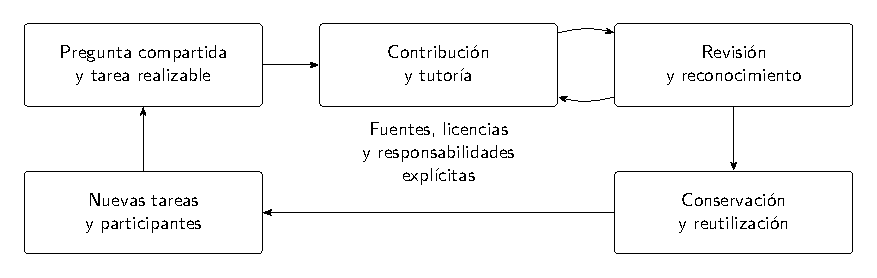
\includegraphics[width=160mm]{figures/modelo.pdf}
\caption{Matriz interpretativa de los casos. La última columna propone comprobaciones de continuidad; no representa tasas observadas de reutilización.}\label{fig:modelo}
\end{figure}

\section{Propuesta de organización}
Una actividad debe definir su unidad mínima de contribución antes de abrir la convocatoria. En un reto de datos puede ser un análisis documentado; en un editatón, una mejora sustentada en fuentes; en una tesis, un resultado reproducible acompañado de interpretación. Esta unidad orienta las tareas, el apoyo necesario y la revisión final. Permite también reconocer traducción, tutoría y documentación, además de programación.

Proponemos un cierre con tres entregas: producto identificable, instrucciones de reutilización y responsable de seguimiento. Para CoAfina, una ficha por proyecto puede enlazar demostración, repositorio, versión, datos y licencia. En el editatón, el identificador de artículo y su historial permiten localizar las contribuciones. En la tesis, memoria y análisis deben enlazarse desde el depósito institucional; el depósito de 2026 de la tesis de Altuve reúne memoria, código con licencia, datos con identificador y entorno ejecutable, y muestra que esa ficha puede completarse años después de la defensa \cite{tesisaltuve}. La apertura se comprueba por componente: la dedicación CC0 de un recurso no se extiende automáticamente a datos externos o dependencias \cite{cc0}.

Retomando las definiciones y metas publicadas de Salud para todos \cite{salud}, la evaluación separa participación, producción, reutilización y continuidad. Una persona activa debe cumplir una acción definida de antemano; finalizar requiere un entregable revisado. La reutilización se documenta mediante una adaptación o ejecución identificable por otra persona. La continuidad puede expresarse mediante nuevas contribuciones o cambios de función, como pasar de participante a mentor. Registrar una revisión a tres y seis meses es una propuesta operativa para próximas actividades, con responsables y fechas establecidos desde el inicio.

\section{Discusión}
Para Venezuela, el punto de entrada puede ser una pregunta local que conecte una asignatura, una comunidad y un conjunto de recursos abiertos. La escala inicial debe corresponder al tiempo de tutoría y revisión disponible. Materiales descargables y tareas asincrónicas permiten acomodar conectividad heterogénea; encuentros breves sirven para resolver dificultades y comparar decisiones. La coordinación requiere compromisos concretos de personas e instituciones, además de visibilidad pública.

La comparación muestra que preservar un producto y sostener una comunidad exigen decisiones diferentes. Un historial permite recuperar una edición, pero la revisión necesita personas; una tesis reconoce un aprendizaje, pero su reutilización necesita acceso al procedimiento. Un hackatón puede abrir una trayectoria si ofrece nuevas responsabilidades y conexiones. En consecuencia, la continuidad debe incorporarse al presupuesto y al reparto de tareas del encuentro.

\paragraph{Alcance y límites} La selección de casos es intencional y cercana a la trayectoria de los autores. Las fuentes describen productos con unidades y períodos distintos; faltan registros comparables por edición y seguimiento longitudinal. La matriz es una síntesis analítica de mecanismos, no una estimación causal del aprendizaje ni una clasificación de eficacia. La equivalencia de cohortes entre las noticias de 2023 permanece sin confirmar. No clasificamos la definición de un formato como más estricta que la de otro.

\section{Conclusiones}
La construcción de comunidades científicas mediante prácticas abiertas requiere conectar tareas realizables, acompañamiento, revisión y conservación. CoAfina, Salud para todos y las experiencias educativas con datos de física permiten examinar esas conexiones desde productos y escalas temporales diferentes. Su valor conjunto no reside en sumar participantes, sino en mostrar decisiones organizativas que pueden explicitarse y adaptarse.

El marco propuesto distingue participación, producción, reutilización y continuidad para evitar que un indicador sustituya a los demás. Para instituciones venezolanas ofrece un punto de partida: seleccionar una pregunta abordable, asignar responsabilidades, preparar materiales reutilizables y documentar qué sucede durante y después de la actividad. La siguiente etapa consiste en aplicar definiciones compartidas y reunir evidencia prospectiva que permita evaluar tanto las oportunidades creadas como sus límites.

\section*{Procedencia y estado del manuscrito}
Este borrador desarrolla el resumen ICHEP 2026 número 668, aceptado como charla y posteriormente retirado según comunicación de los autores por imposibilidad de asistencia. El arbitraje del resumen no constituye arbitraje de este texto. Se citan los antecedentes publicados y no se reivindican sus resultados como inéditos. La validación de autoría, afiliaciones, financiación, conflictos de interés y direcciones de correspondencia permanece pendiente de revisión de los autores. El registro de evidencia se incluye en el repositorio acompañante.


\begin{thebibliography}{99}\small\setlength{\itemsep}{2pt}\setlength{\parskip}{0pt}
\bibitem{unesco}UNESCO. Recomendación sobre la Ciencia Abierta. París (2021). \url{https://www.unesco.org/en/legal-affairs/recommendation-open-science}.

\bibitem{wenger}Wenger, E. \emph{Communities of Practice: Learning, Meaning, and Identity}. Cambridge University Press (1998). \url{https://doi.org/10.1017/CBO9780511803932}.

\bibitem{hacklearning}Schulten, C. y Chounta, I.-A. How do we learn in and from Hackathons? A systematic literature review. \emph{Education and Information Technologies} \textbf{29}, 20103--20134 (2024). \url{https://doi.org/10.1007/s10639-024-12668-1}.

\bibitem{hackmapping} Costa, G., García-Holgado, A. y Alvarez, P. Systematic mapping of the literature on hackathons. \emph{Frontiers in Education} \textbf{10}, 1701443 (publicado el 22 de enero de 2026). \url{https://doi.org/10.3389/feduc.2025.1701443}.

\bibitem{coafina}Camacho Toro, R., Briceño, Y. y Martínez, A. Hackathon Co-Afina 2023: Latin American Students Drive Innovation with Open Data. Software Sustainability Institute (7 de diciembre de 2023). \url{https://www.software.ac.uk/blog/hackathon-co-afina-2023-latin-american-students-drive-innovation-open-data}.

\bibitem{coafina2024}Briceño, Y. CoAfina returns: The Latin American hackathon focused on open data. LA-CoNGA physics (30 de mayo de 2024). \url{https://laconga.redclara.net/en/coafina-returns-the-latin-american-hackathon-focused-on-open-data/}.

\bibitem{salud}Sánchez, A., Bennett, A., Stifano, A., Peña-Rosas, J.P. y Mehta, S. Editatón Salud para todos: modelo participativo de traducción del conocimiento y movilización comunitaria en Wikipedia. \emph{Archivos Latinoamericanos de Nutrición} \textbf{76}(1), 49--56 (2026). \url{https://doi.org/10.37527/2026.76.1.006}.

\bibitem{atlas}Sánchez Pineda, A. Boosting high-energy physics education around the world with ATLAS Open Data. ATLAS/CERN (26 de julio de 2018). \url{https://atlas.cern/updates/blog/HEP-education-worldwide-with-atlas-open-data}.

\bibitem{coafinacontinuidad}Briceño, Y. Latin American students develop innovative solutions with open data at Co-Afina 2023. LA-CoNGA physics (30 de noviembre de 2023). \url{https://laconga.redclara.net/en/latin-american-students-develop-innovative-solutions-with-open-data-at-co-afina-2023/}.

\bibitem{wikihealth}Heilman, J.M., Kemmann, E., Bonert, M. y colaboradores. Wikipedia: A Key Tool for Global Public Health Promotion. \emph{Journal of Medical Internet Research} \textbf{13}(1), e14 (2011). \url{https://doi.org/10.2196/jmir.1589}.

\bibitem{openglam}OpenGLAM. Effective Open Data \& Soft: Knowledge Transfer that Boosts Computer Skills in the Americas. Anuncio de conferencia de Arturo Sánchez, 27 de abril de 2020. \url{https://openglam.at/arturo_sanchez/}.

\bibitem{hsftraining}Malik, S., Meehan, S., Lieret, K. y colaboradores. Software Training in HEP. \emph{Computing and Software for Big Science} \textbf{5}, 22 (2021). \url{https://doi.org/10.1007/s41781-021-00069-9}. Versión de autor: \url{https://arxiv.org/abs/2103.00659}.

\bibitem{cc0}Creative Commons. Public Domain: CC0 Public Domain Dedication. Documentación institucional. Consulta: 21 de octubre de 2026. \url{https://creativecommons.org/public-domain/}.
\end{thebibliography}

\end{document}
